\section{问题一:关系模型的建立与求解}
为识别影响男胎 Y 染色体浓度的主要因素并量化其作用,我们先构建最终数据集,再通过探索性分析与迭代建模建立能反映数据规律的关系模型。具体流程见 \cref{fig:关系模型的建立与求解流程}。

\begin{figure}[h!]
    \centering
    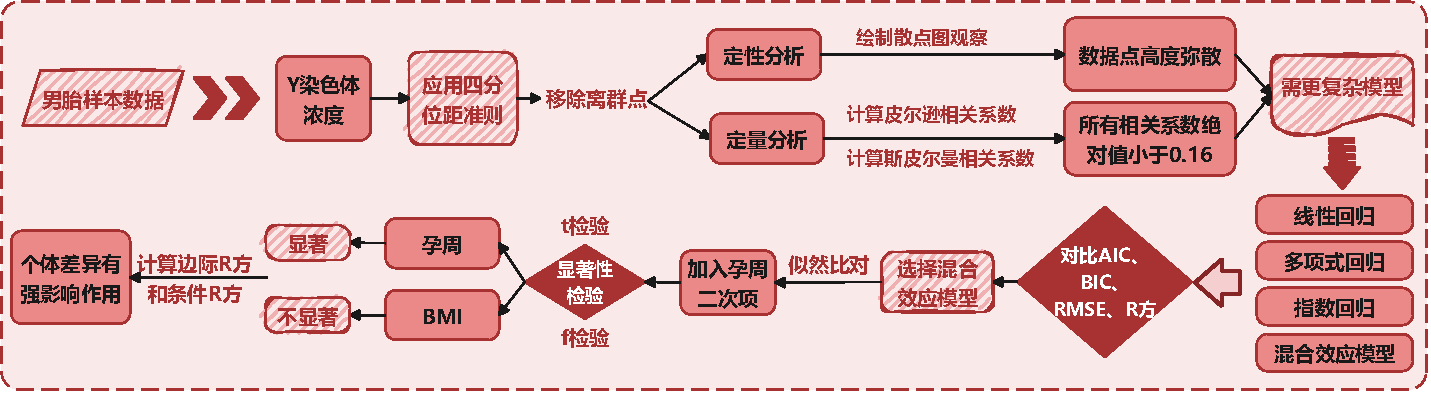
\includegraphics[width=\textwidth]{figs/3问题一/问题一.pdf}
    \caption{关系模型的建立与求解流程}
    \label{fig:关系模型的建立与求解流程}
\end{figure}

\subsection{数据准备与探索性分析}
分析始于一份经过初步处理的男胎样本数据。为保证后续建模的稳定,我们对Y染色体浓度这个核心变量应用了四分位距法进行离群点检测。在联合筛选标准下,部分包含极端值的样本记录被移除,最终形成了一个用于建模的分析数据集。

\begin{figure}[h!]
\centering
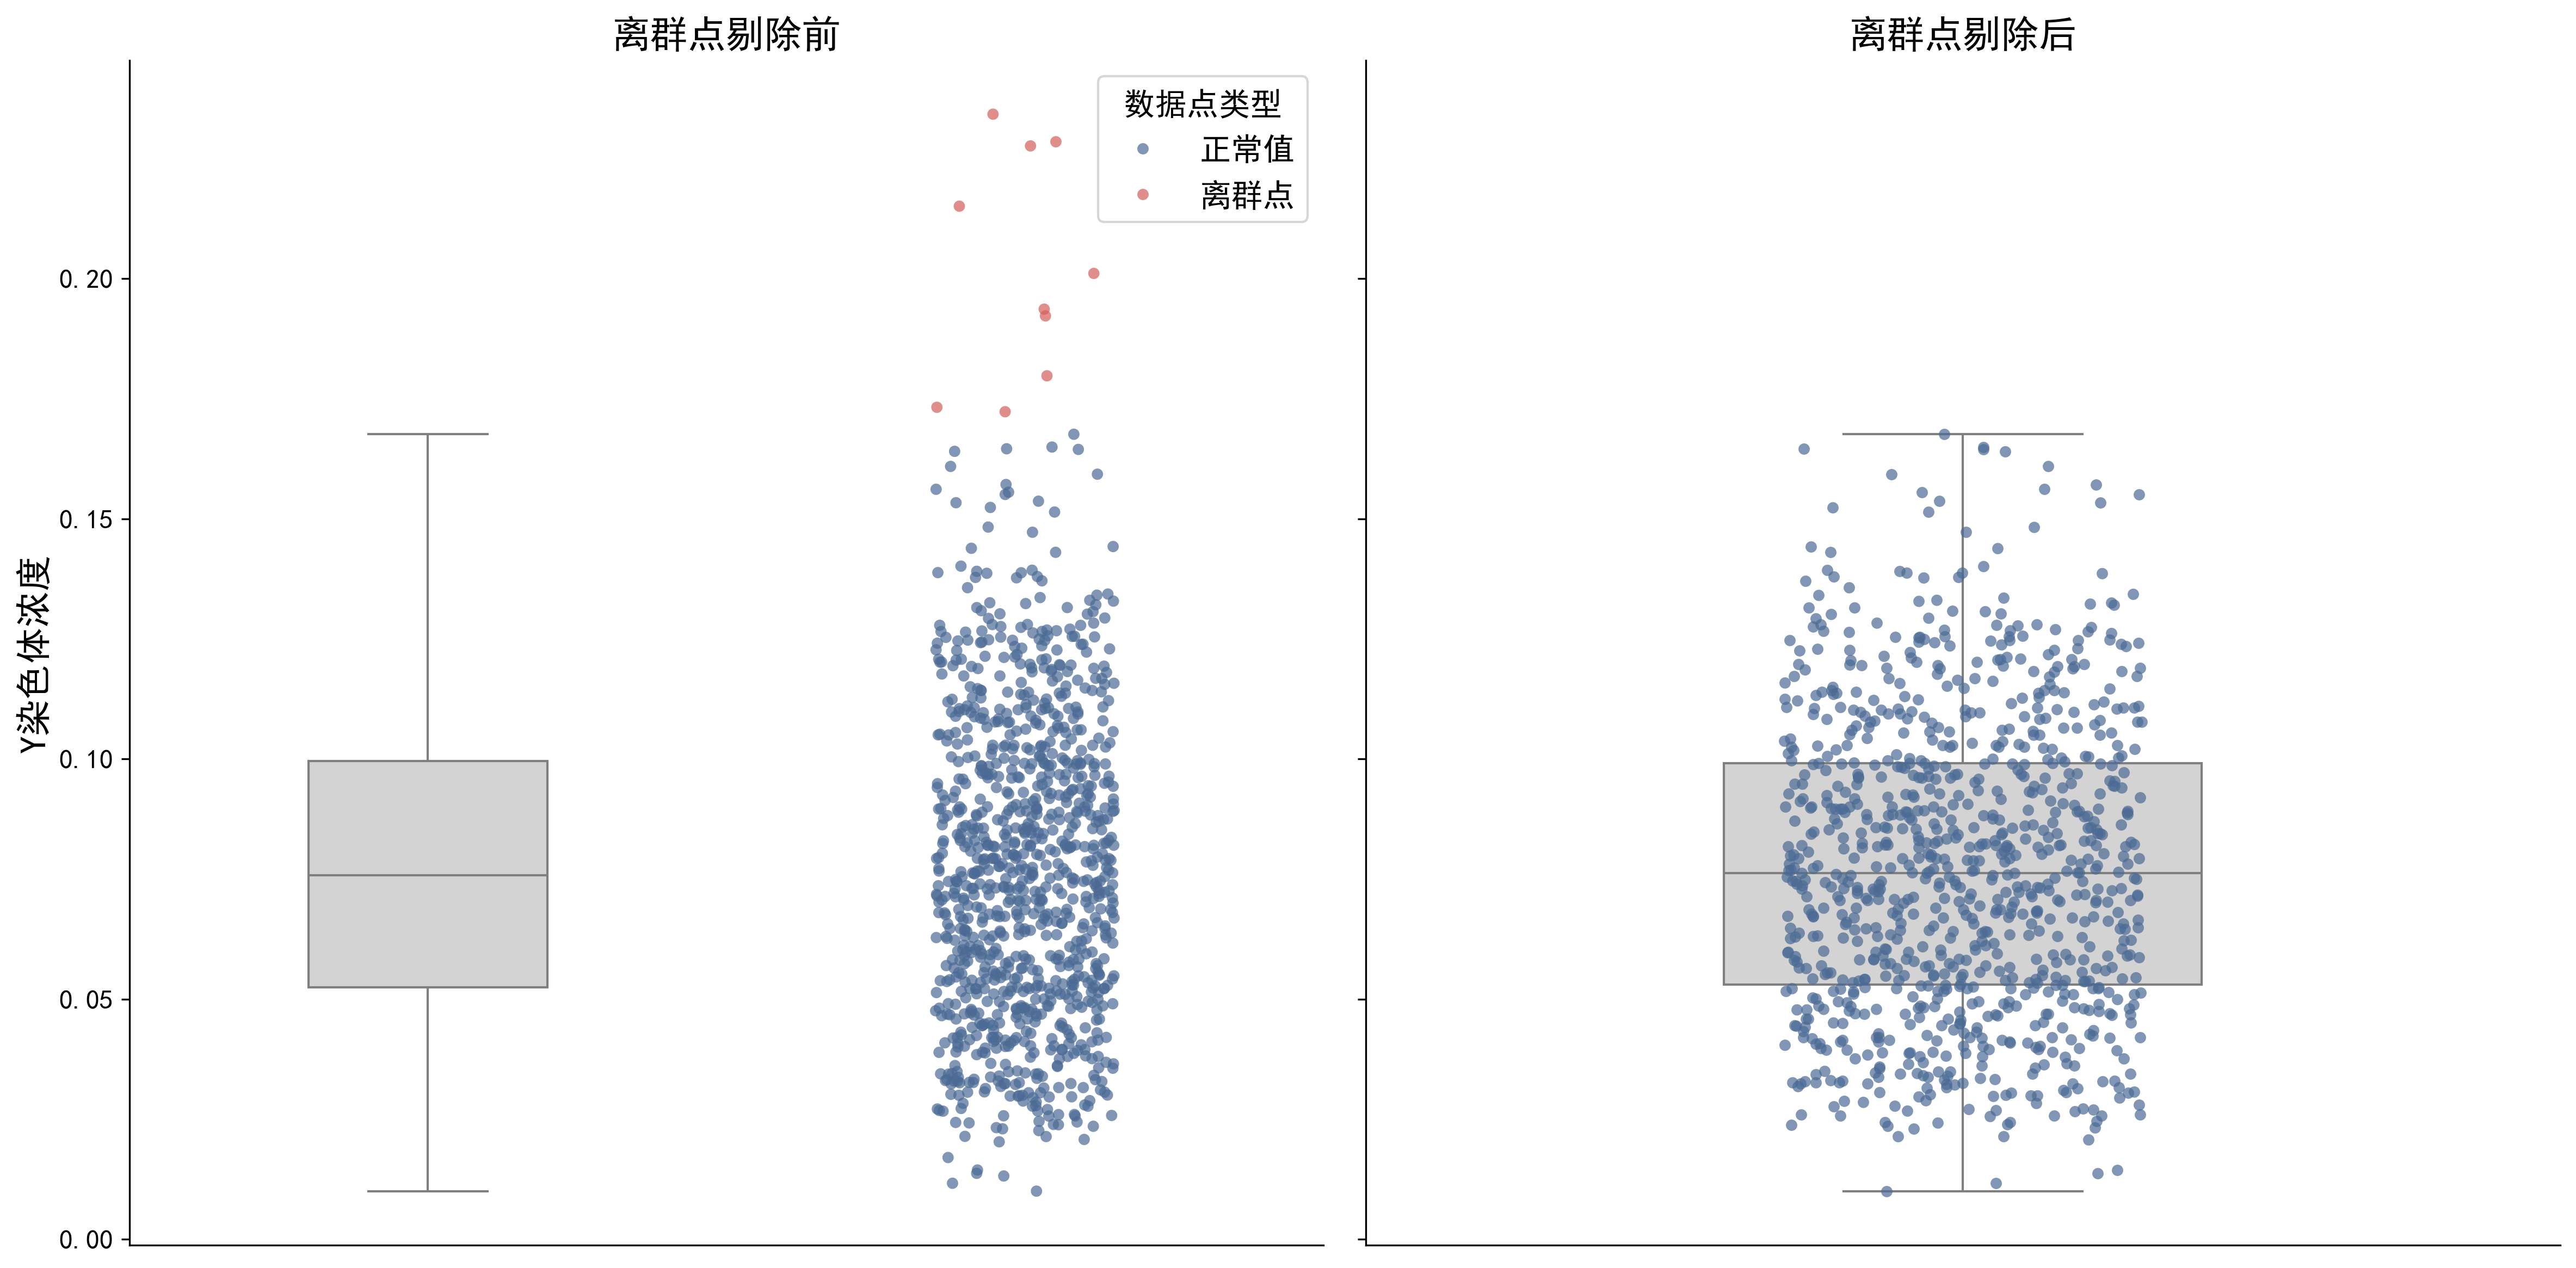
\includegraphics[width=\textwidth]{figs/3问题一/Y浓度离群点剔除可视化.png}
\caption{Y染色体浓度数据离群点剔除前后对比}
\label{fig:outlier_removal}
\end{figure}

\cref{fig:outlier_removal}为数据清洗过程的可视化结果,其对比了Y染色体浓度在离群点剔除前后的数据分布,被识别为离群点的数据点以不同颜色标记,清洗后的数据分布更为集中,减少了极端值对模型估计的潜在干扰。

在正式建模之前,我们对清洗后的数据进行了探索性分析。通过绘制Y染色体浓度与孕周、孕妇BMI的散点图,我们对变量间的关系形态进行了初步探查,如\cref{fig:scatter_plots}所示。

\begin{figure}[h!]
\centering
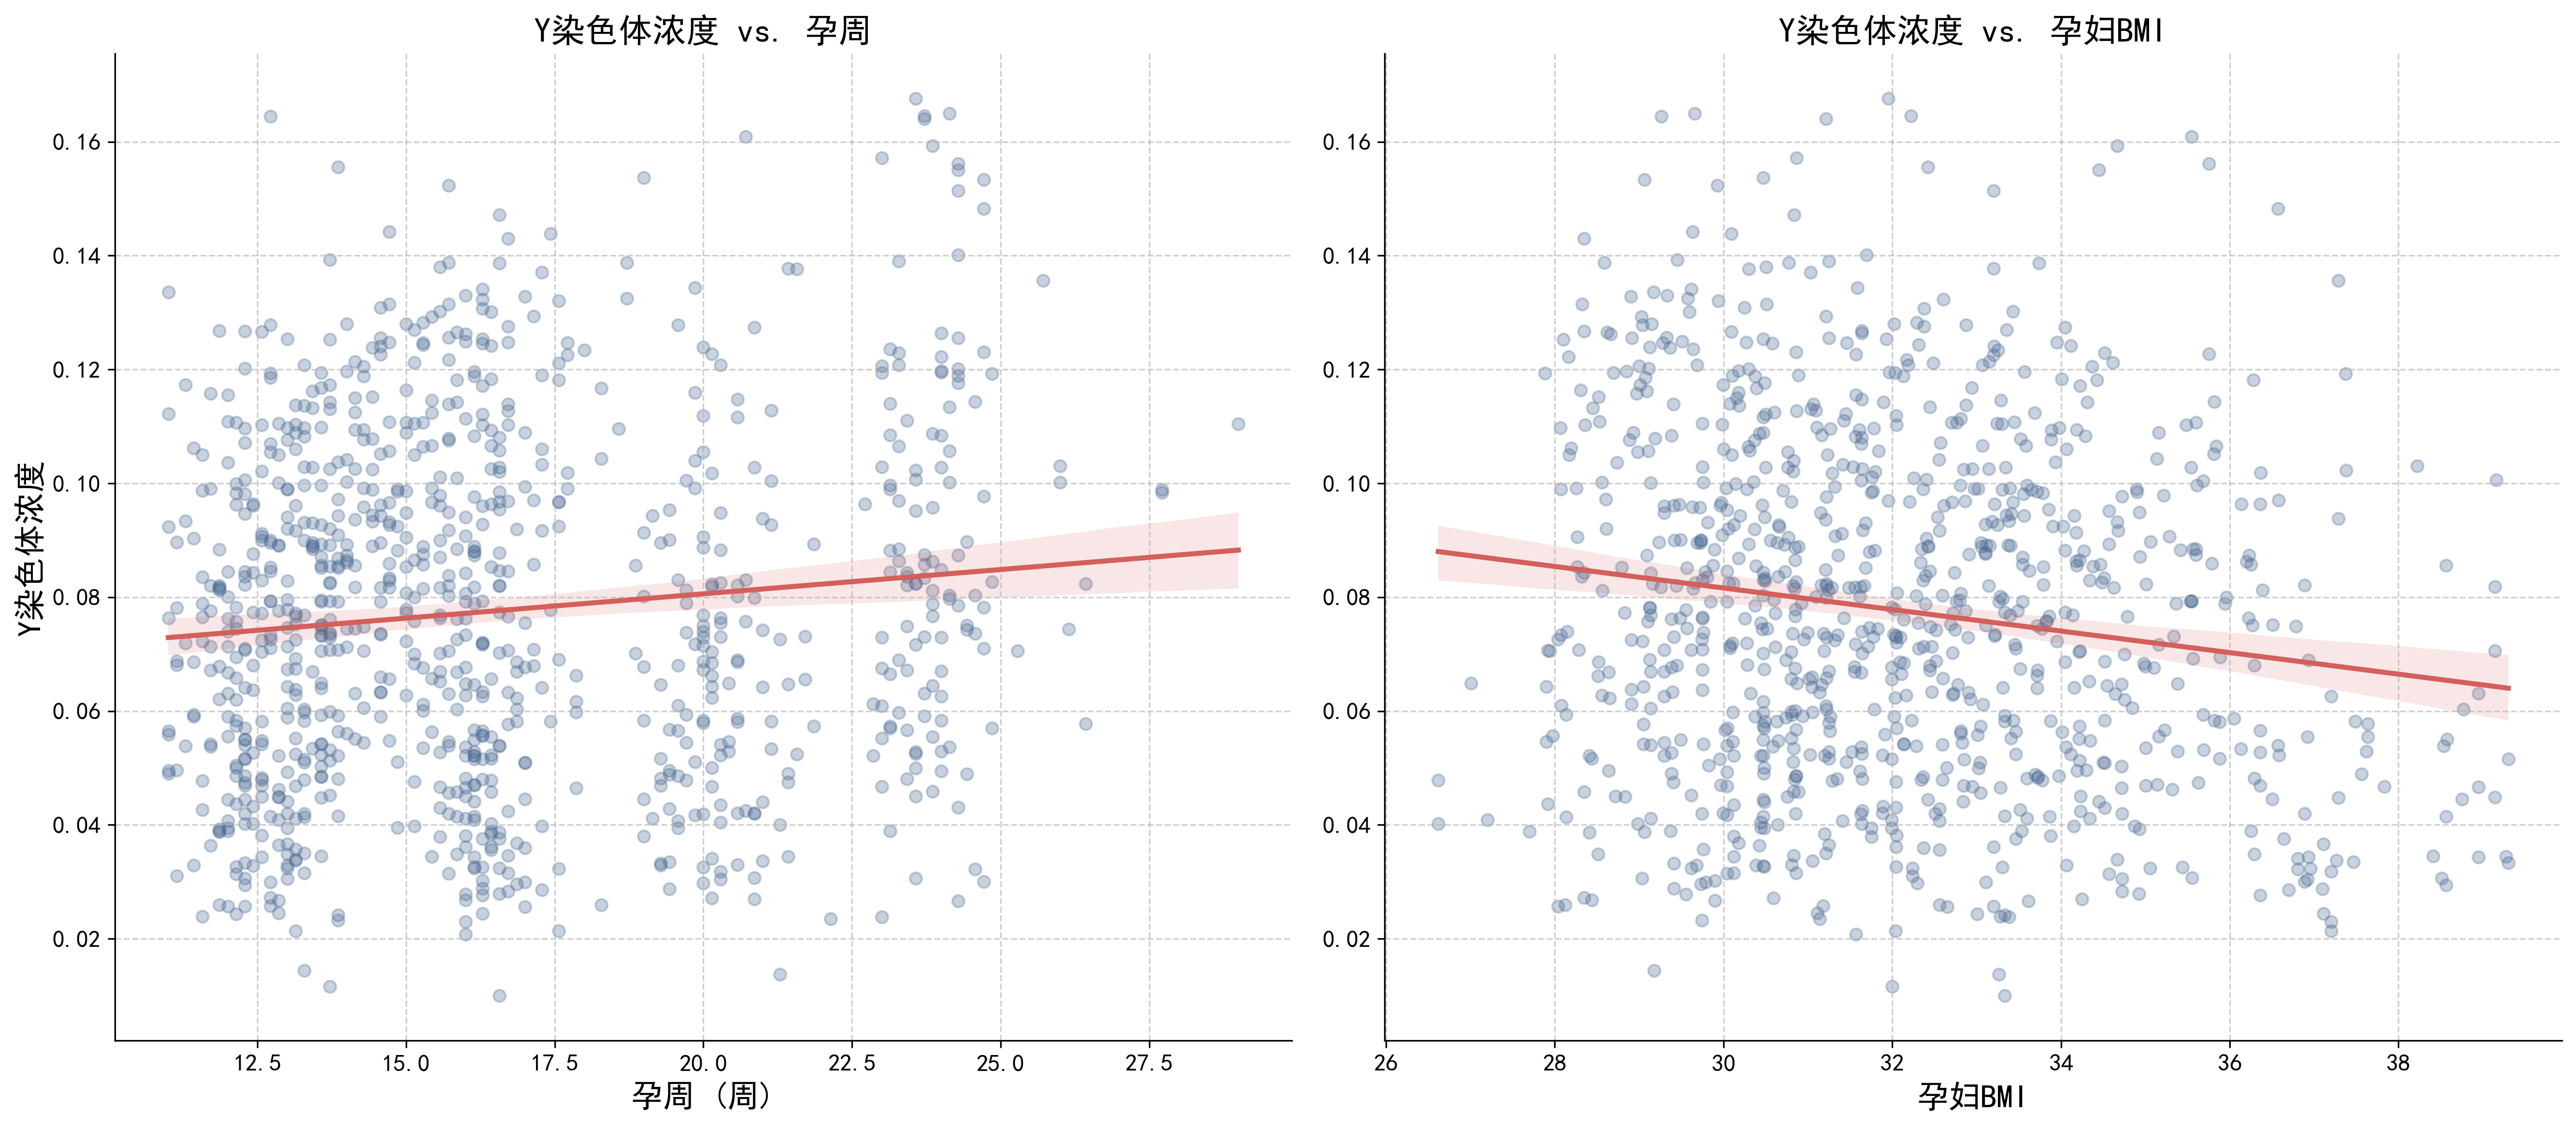
\includegraphics[width=1\textwidth]{figs/3问题一/Y浓度_vs_变量_散点图.png}
\caption{Y染色体浓度与孕周及BMI的散点关系图}
\label{fig:scatter_plots}
\end{figure}

根据\cref{fig:scatter_plots},Y染色体浓度与孕妇BMI的散点分布较为弥散,未呈现出特定的线性或非线性模式。而Y染色体浓度与孕周的散点图则呈现出一种微弱的U型曲线趋势,表明两者之间可能存在非线性关系。为量化变量间的关联强度,我们计算了皮尔逊与斯皮尔曼相关系数。皮尔逊相关系数用以衡量线性关联,其计算公式为
\begin{equation}
r = \frac{\sum_{i=1}^{n}(x_i - \bar{x})(y_i - \bar{y})}{\sqrt{\sum_{i=1}^{n}(x_i - \bar{x})^2} \sqrt{\sum_{i=1}^{n}(y_i - \bar{y})^2}}
\end{equation}

斯皮尔曼相关系数则用以衡量单调关系,计算公式为
\begin{equation}
\rho = 1 - \frac{6 \sum_{i=1}^{n} d_i^2}{n(n^2 - 1)}
\end{equation}

计算结果汇总于\cref{tab:correlation}。

\begin{table}[h!]
\centering
\caption{Y染色体浓度与孕周、BMI的相关性分析}
\label{tab:correlation}
\begin{tabular}{lcc}
\hline
变量对 & 皮尔逊相关系数 $r$ & 斯皮尔曼相关系数 $\rho$ \\
\hline
浓度 vs 孕周 & 0.1087 & 0.0851 \\
浓度 vs BMI & -0.1531 & -0.1321 \\
\hline
\end{tabular}
\end{table}

\cref{tab:correlation}的数据显示,Y染色体浓度与孕周、BMI的线性相关性均较弱,这与散点图的观察结果一致,并进一步说明简单的线性模型可能不足以描述变量间的复杂关系。

\subsection{关系模型的构建与择优}
基于探索性分析的发现,我们构建了四种不同复杂度的模型来拟合Y染色体浓度、孕周与BMI之间的关系,并通过统计指标对它们进行比较,以选取最合适的模型。

模型一为多元线性回归模型,作为后续比较的基准。其形式为
\begin{equation}
Y_{ij} = \beta_0 + \beta_1 GW_{ij} + \beta_2 BMI_{ij} + e_{ij}
\end{equation}

模型二为多元多项式回归模型,用以捕捉潜在的非线性关系。其形式为
\begin{equation}
Y_{ij} = \beta_0 + \sum_{k=1}^p \beta_k GW_{ij}^k + \sum_{l=1}^q \gamma_l BMI_{ij}^l + e_{ij}
\end{equation}

模型三为多元指数回归模型,通过对数变换处理可能的指数增长关系。其形式为
\begin{equation}
\ln(Y_{ij}) = \beta_0 + \beta_1 GW_{ij} + \beta_2 BMI_{ij} + e_{ij}
\end{equation}

考虑到数据中可能存在同一孕妇的多次检测记录,孕妇个体间的差异可能对Y染色体浓度有较大影响。因此,我们引入了非线性混合效应模型,即模型四。该模型在多项式回归的基础上,为每个孕妇个体设置了随机效应项,以解释个体间的异质性。其通用形式为
\begin{equation}
Y_{ij} = (\beta_0 + u_{0i}) + \sum_{k=1}^p \beta_k GW_{ij}^k + \sum_{l=1}^q \gamma_l BMI_{ij}^l + e_{ij}
\end{equation}
其中 $u_{0i}$ 服从均值为0的正态分布,代表第 $i$ 位孕妇的个体效应。

为在上述模型中进行选择,我们计算了各自的对数似然值、赤池信息准则AIC、贝叶斯信息准则BIC、均方根误差RMSE和决定系数$R^2$,评估指标对比见\cref{tab:model_comparison}。

\begin{table}[h!]
\centering
\caption{四种候选模型的评估指标对比}
\label{tab:model_comparison}
\resizebox{\columnwidth}{!}{
\begin{tabular}{lccccc}
\hline
模型 & 对数似然值 & AIC & BIC & RMSE & $R^2$ \\
\hline
M1 线性回归 & 1999.22 & -3992.43 & -3977.82 & 0.0303 & 0.0377 \\
M2 多项式回归 & 1999.61 & -3991.23 & -3971.75 & 0.0303 & 0.0375 \\
M3 指数回归 & -573.15 & 1152.29 & 1166.90 & 0.0310 & 0.0376\\
M4 混合效应模型 & 2367.64 & -4719.27 & -4680.32 & 0.0326 & 边际:0.4052, 条件:0.9160 \\
\hline
\end{tabular}}
\end{table}

\cref{tab:model_comparison}的评估结果显示,模型一、二、三的决定系数均低于0.04,说明这些模型对Y染色体浓度变异的解释能力非常有限。相比之下,模型四的对数似然值最高,AIC和BIC值最低,显示出更优的拟合度。

\begin{figure}[h!]
\centering
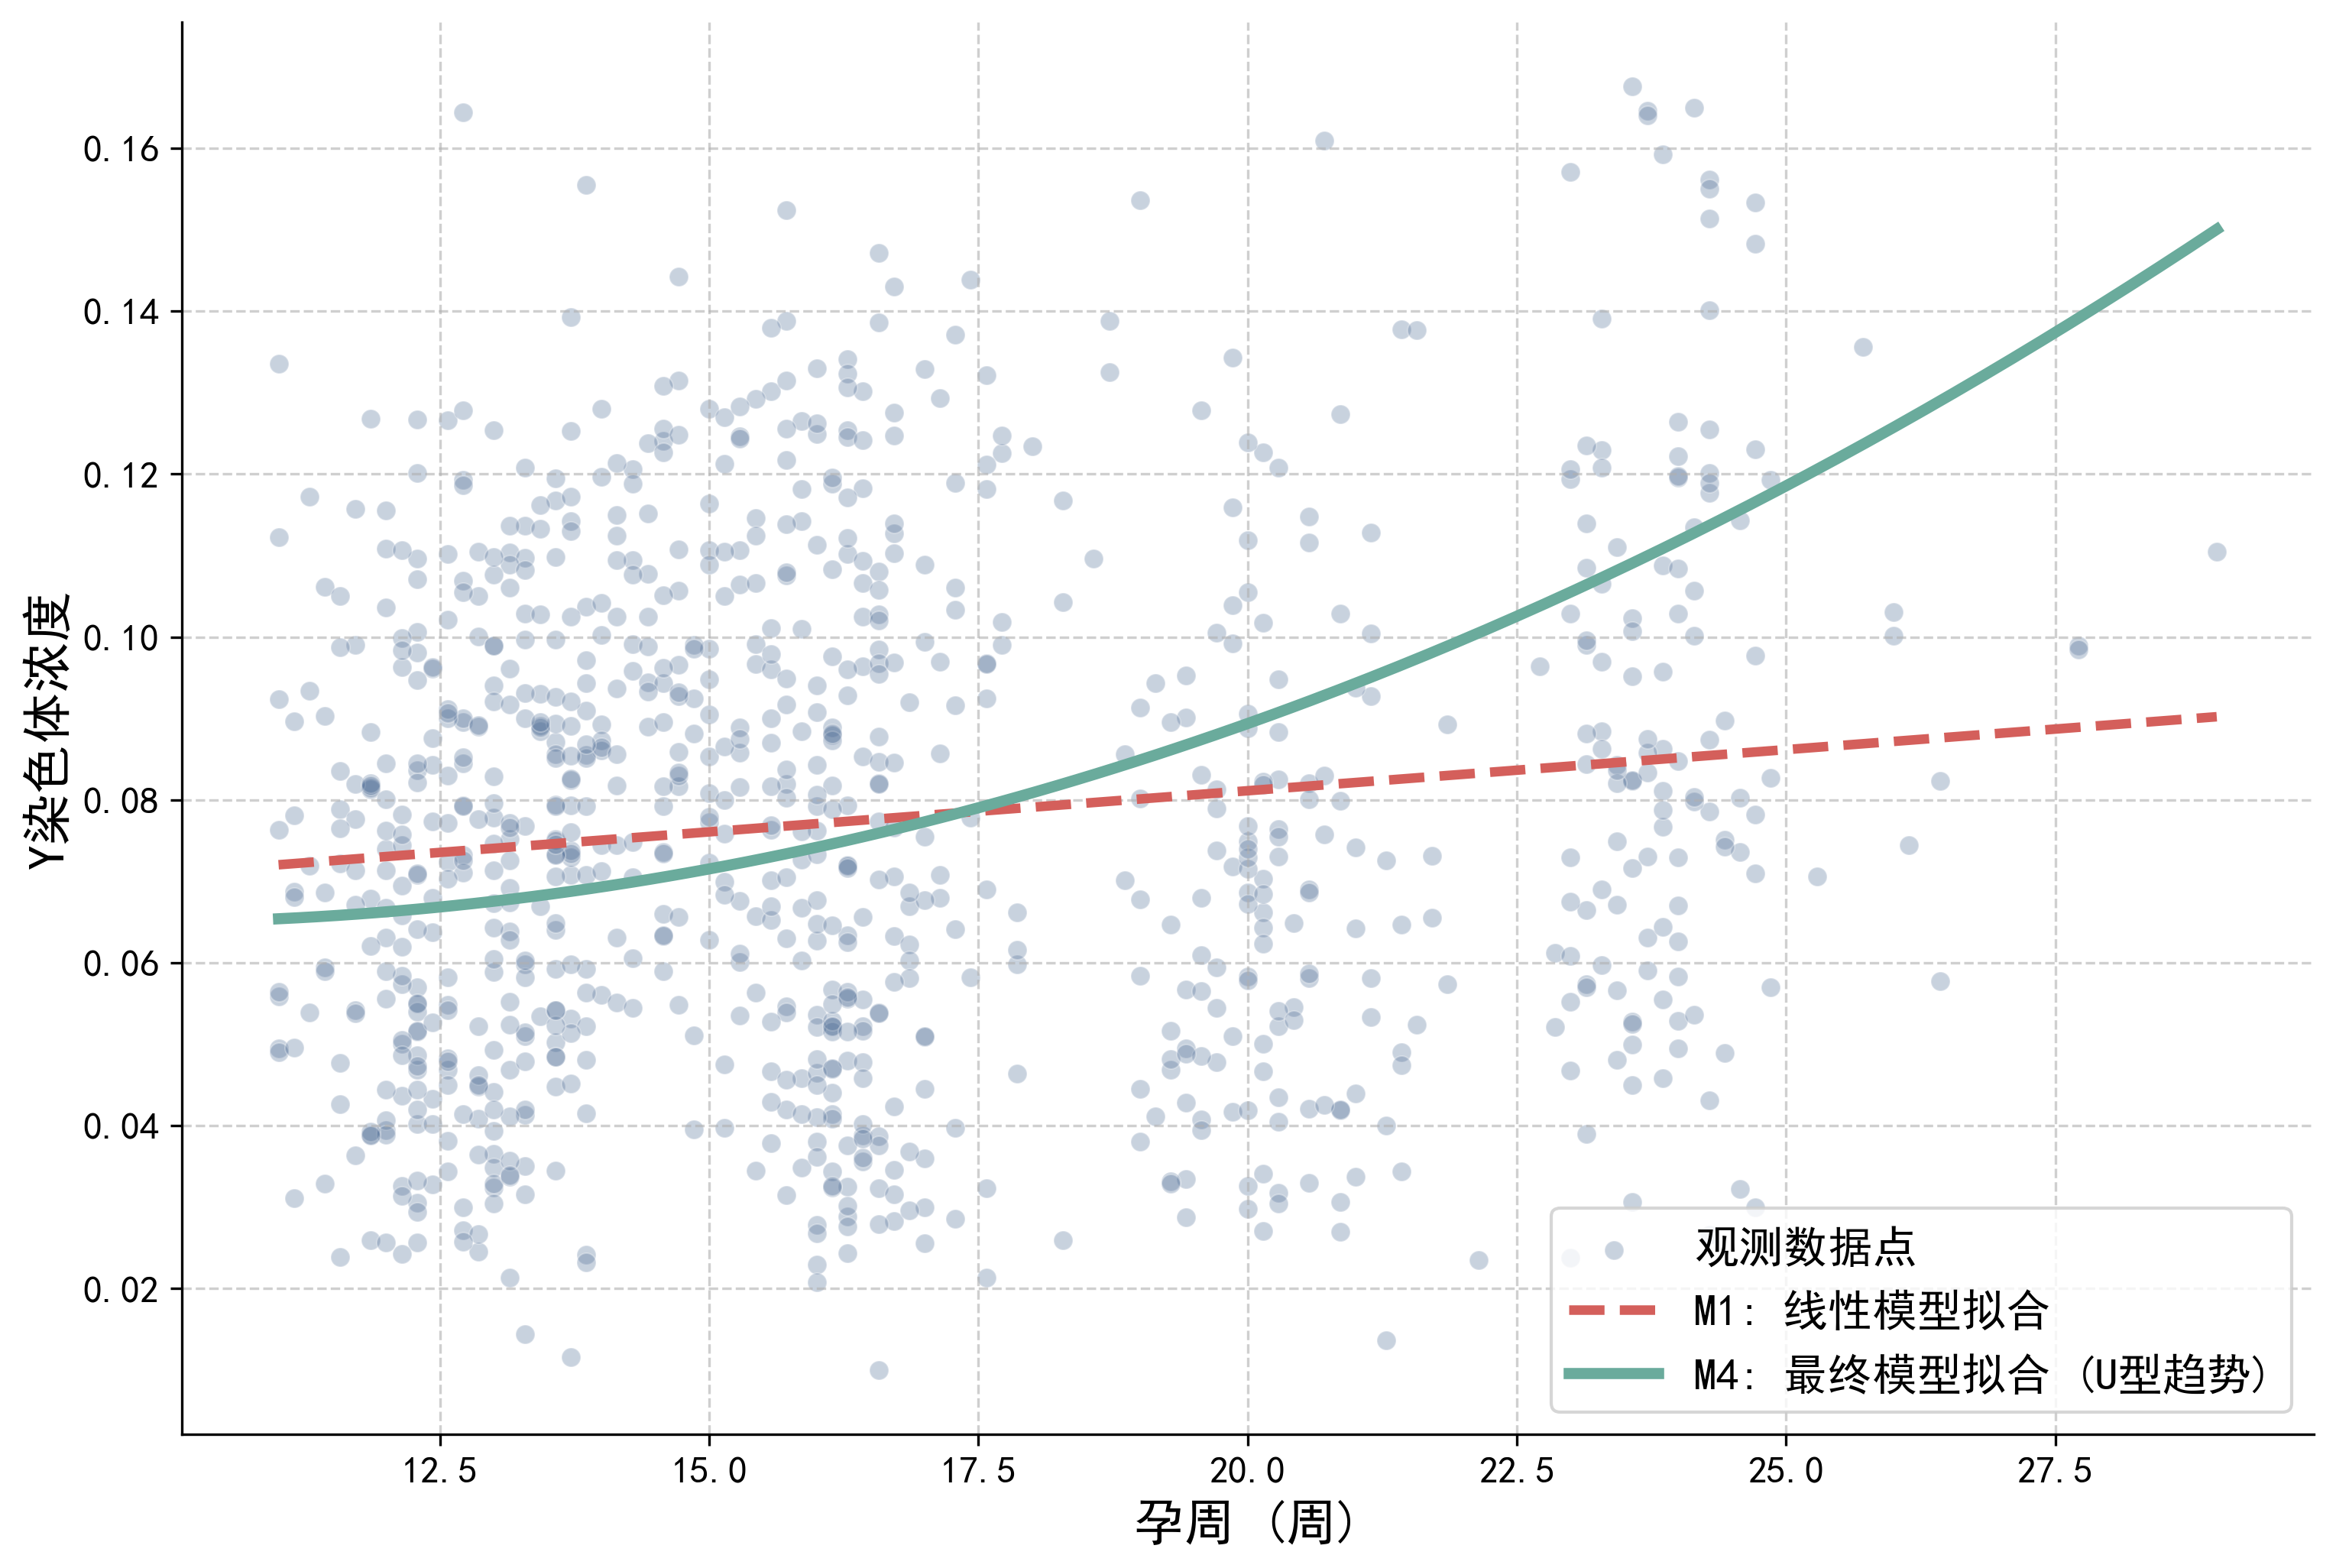
\includegraphics[width=0.9\textwidth]{figs/3问题一/模型拟合效果对比图.png}
\caption{线性模型与非线性混合效应模型拟合效果对比}
\label{fig:fit_comparison}
\end{figure}

\cref{fig:fit_comparison}对比了线性模型与非线性模型对数据趋势的拟合情况。非线性模型所捕捉的U型曲线趋势比线性模型更能贴合数据的整体分布形态。基于上述分析,我们最终选择非线性混合效应模型作为描述Y染色体浓度与母体指标关系的模型。

\subsection{最终模型解析与显著性检验}
在确定采用非线性混合效应模型后,我们通过似然比检验对其具体形式进行了优化。检验结果表明,在模型中加入孕周的二次项能提升模型拟合度,而加入BMI的二次项及孕周与BMI的交互项则无改善。因此,最终确立的模型形式为
\begin{equation}
Y_{ij} = (\beta_0 + u_{0i}) + ((\beta_1 + u_{1i})GW_{ij} + \beta_2 GW_{ij}^2) + \gamma_1 BMI_{ij} + e_{ij}
\end{equation}
其中,$u_{0i}$ 和 $u_{1i}$ 分别代表第 $i$ 位孕妇的随机截距和随机斜率。为检验模型中各变量的效应,我们对模型系数进行了t检验。其原假设为系数等于零,统计量计算公式为
\begin{equation}
t = \frac{\hat{\beta}_k - 0}{SE(\hat{\beta}_k)}
\end{equation}

同时,我们通过F检验来评估模型整体的显著性,其原假设为所有自变量系数同时为零,统计量计算公式为
\begin{equation}
F = \frac{SSR/k}{SSE/(n-k-1)}
\end{equation}

最终模型固定效应参数的估计与检验结果如\cref{tab:fixed_effects}所示。

\begin{table}[h!]
\centering
\small
\caption{最终模型固定效应参数估计与检验}
\label{tab:fixed_effects}
\begin{tabular}{lcccccc}
\hline
变量 & 系数 & 标准误 & z值 & p值 & 95\%置信区间下限 & 95\%置信区间上限 \\
\hline
Intercept & 0.1188 & 0.0217 & 5.471 & $<$0.001 & 0.0762 & 0.1613 \\
孕周 & -0.0044 & 0.0012 & -3.639 & 0.0003 & -0.0067 & -0.0020 \\
孕妇BMI & -0.0010 & 0.0006 & -1.670 & 0.0949 & -0.0022 & 0.0002 \\
孕周二次项 & 0.0002 & 3.47e-05 & 6.532 & $<$0.001 & 0.0002 & 0.0003 \\
\hline
\end{tabular}
\end{table}

\cref{tab:fixed_effects}的参数估计结果显示,孕周项的系数显著为负,而其二次项的系数显著为正,这共同确认了Y染色体浓度随孕周呈现先下降后上升的U型非线性关系。截距项也表现出高度显著性。孕妇BMI项的p值为0.0949,在0.05的显著性水平下不显著,表明其对Y染色体浓度的影响不稳定。

\begin{table}[h!]
\centering
\caption{最终模型决定系数}
\label{tab:r_squared}
\begin{tabular}{lc}
\hline
指标 & 值 \\
\hline
边际 $R^2$ & 0.4052 \\
条件 $R^2$ & 0.9160 \\
\hline
\end{tabular}
\end{table}

模型的决定系数分析见\cref{tab:r_squared}。边际$R^2$为0.4052,表示由孕周和BMI所代表的固定效应可以解释约40.5\%的变异。条件$R^2$为0.9160,表示在模型同时考虑固定效应和个体随机效应后,总共能解释91.6\%的变异。这两个$R^2$值的差异,印证了个体差异性在Y染色体浓度变化中起主导作用。

\begin{figure}[h!]
\centering
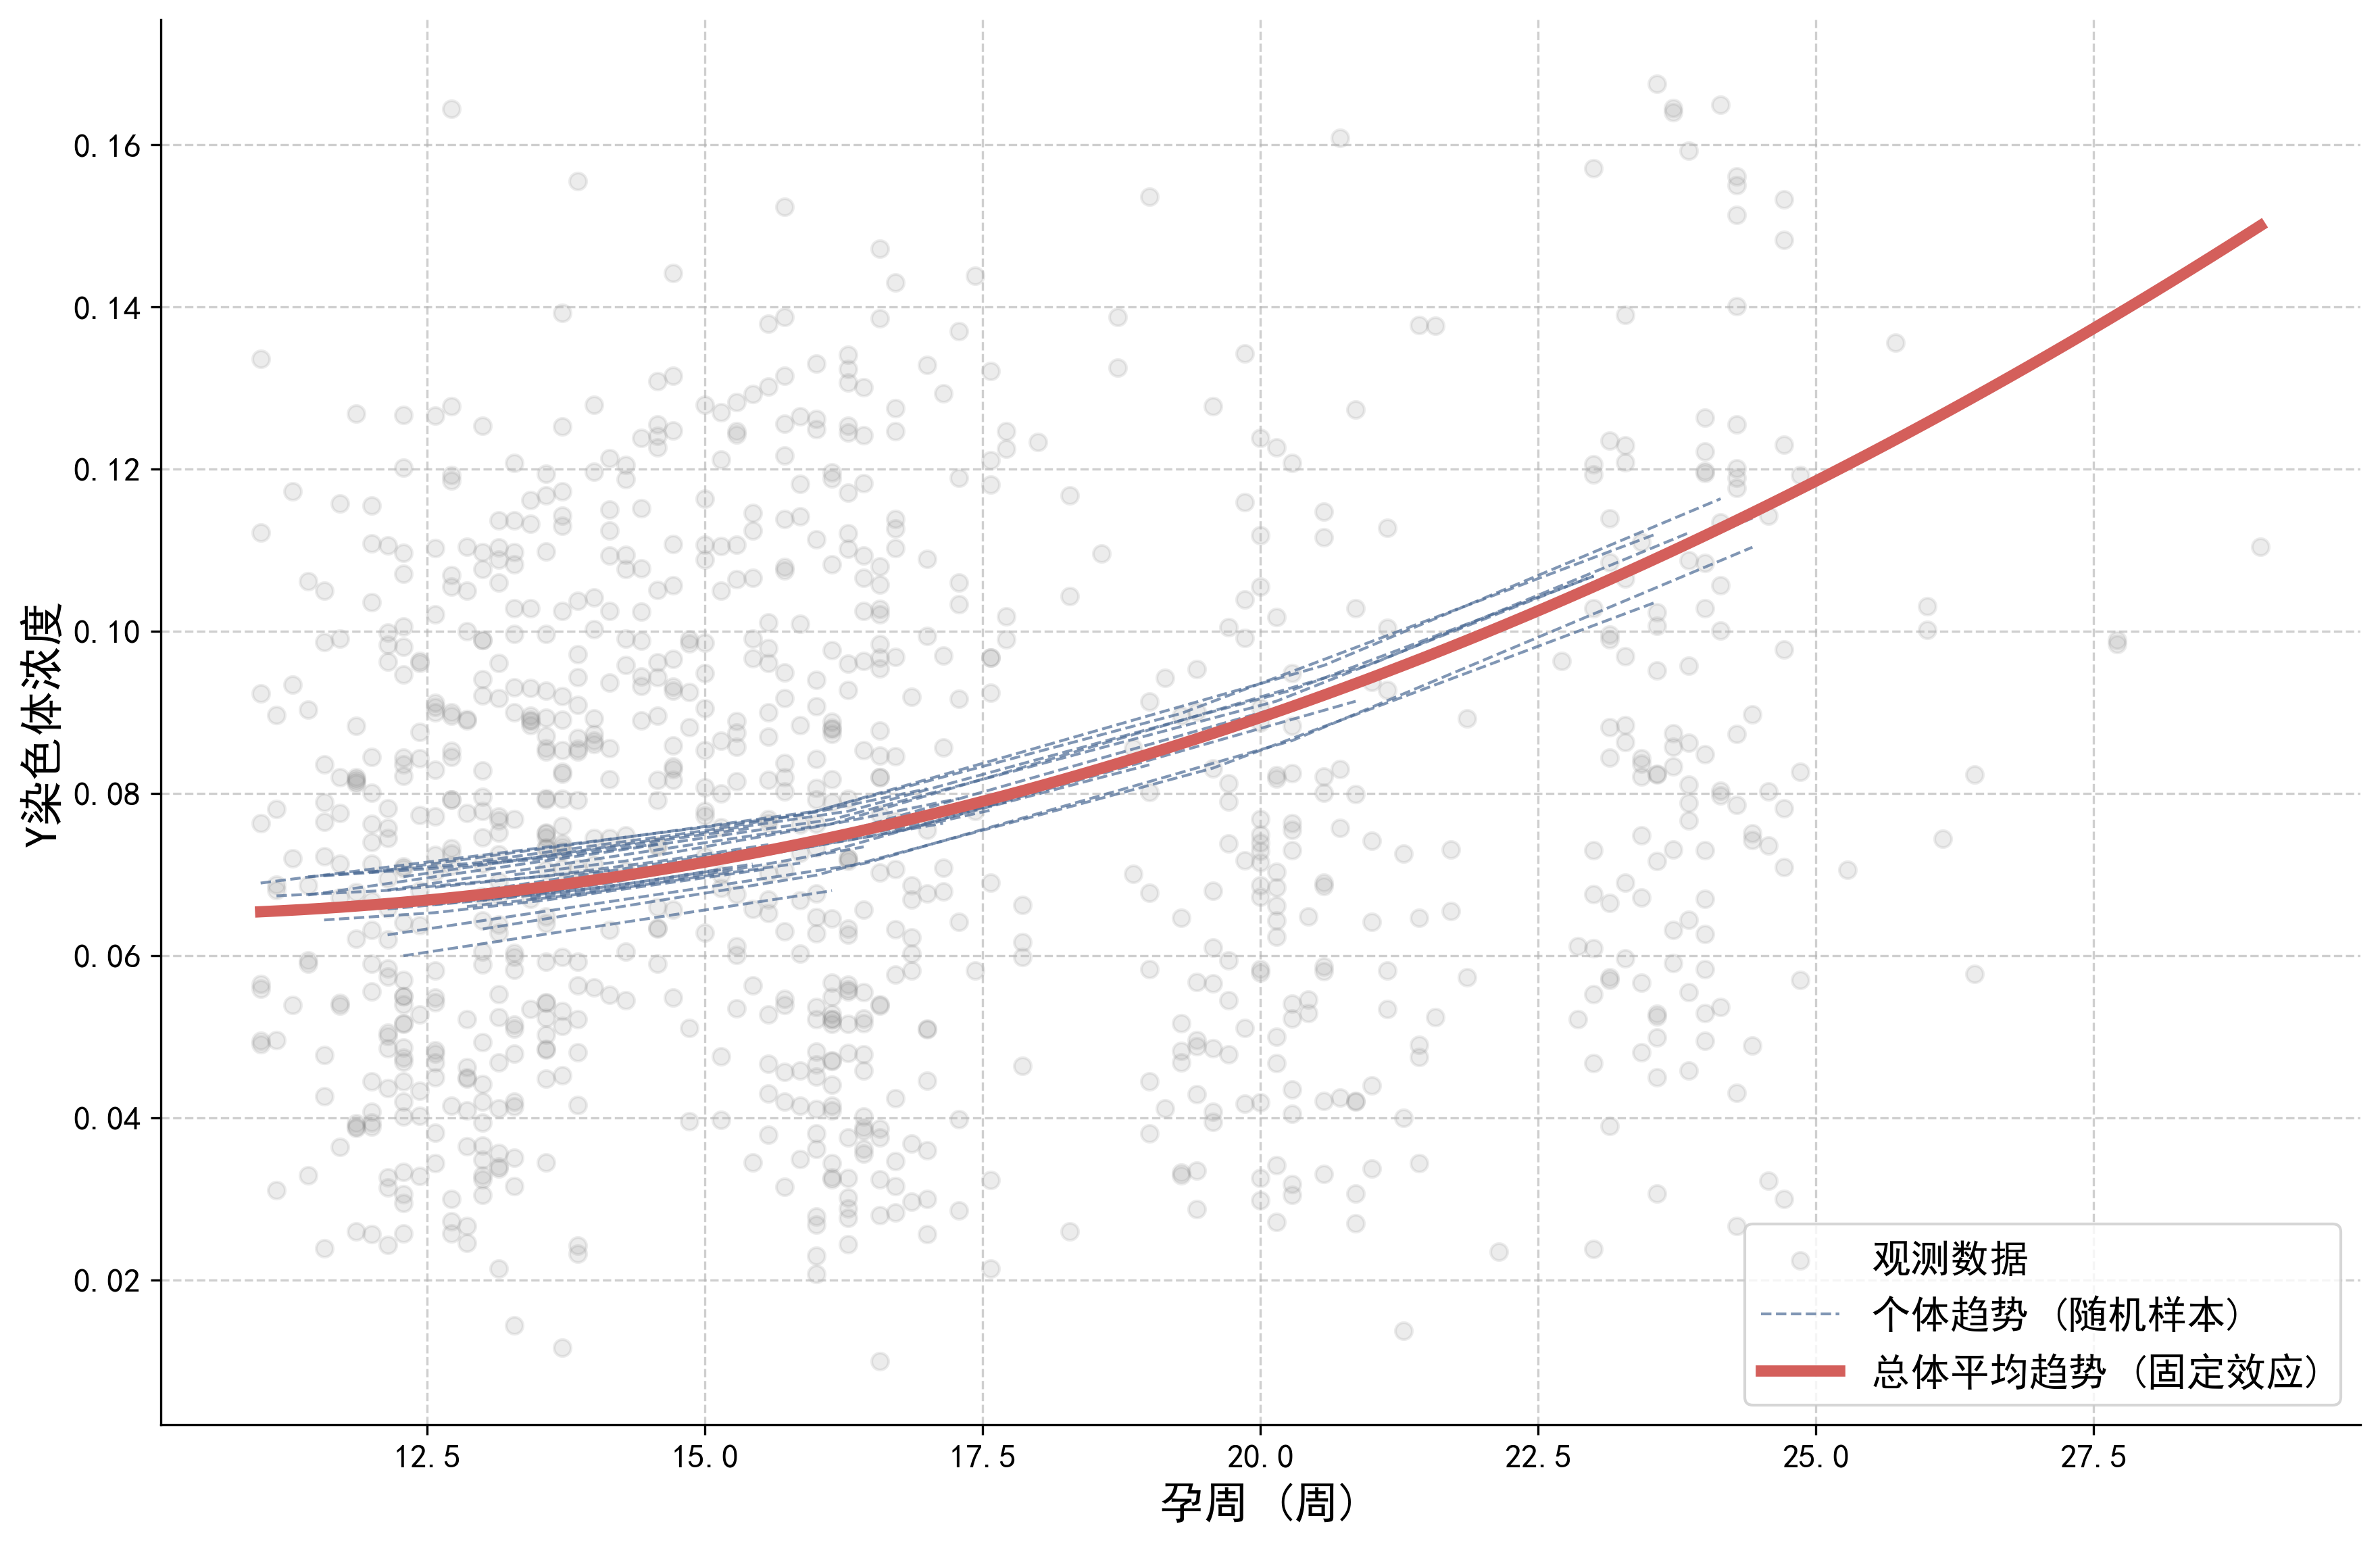
\includegraphics[width=\textwidth]{figs/3问题一/最终模型M4_可视化.png}
\caption{最终模型揭示的总体趋势与个体差异}
\label{fig:final_model_viz}
\end{figure}

\cref{fig:final_model_viz}是最终模型结果的可视化呈现。图中的红色实线代表了由固定效应决定的平均变化趋势,即总体样本共有的U型规律。大量的蓝色虚线则代表了考虑随机效应后,每一位孕妇个体的实际变化轨迹。

综合上述分析,可以得出Y染色体浓度变化规律的结论。其变化遵循一个由孕周主导的U型非线性模式,即浓度随孕周增加先发生下降,后转为上升,这一趋势具有统计学上的显著性。然而,这一普遍规律在不同孕妇个体间的表现存在巨大差异,个体独特性是引起浓度变化的更主要来源。相比之下,孕妇的BMI指标在此模型中未表现出稳定的影响。
